\documentclass{article}

\usepackage{times}
\usepackage{amsmath}
\usepackage{graphicx}
\usepackage{hyperref}

\begin{document}

\section{ZT37 VSD Compressor Minimum Flow Compression}
At minimum speed of VSD operation the first stage of compression operates as follows:

\begin{itemize}
\item Ambient Temperature: 300K (Assumed)
\item Ambient Pressure: 101,325 Pa (Assumed)
\item Compressed Air Flow Rate: 87.2 acfm (CAGI Data sheet: equivalent to 0.0412 $m^{3} / s$)
\item Element 1 Outlet Pressure: 2.5 barg
\end{itemize}

We can normalise to standard temperature and pressure we can calculate the number of moles of air being compressed. This is useful when applying the ideal gas equation:

\begin{equation}
PV = nRT
\label{eq:idealgas}
\end{equation}

\begin{equation}
\frac{P_{1}V_{1}}{T_{1}}  = \frac{P_{2}V_{2}}{T_{2}}
\label{eq:combinedgaslaw}
\end{equation}

\begin{equation}
V_{2} = \frac{101,325 * 0.0412 * 273.15}{300*100,000} = 0.038 m^{3}
\end{equation}

One mole of gas occupies 22.7 l at standard temperature of pressure.

\begin{equation}
\frac{0.038}{.0227} = 1.67 \text{moles}
\end{equation}

\section{Isothermal Compression}
For isothermal compression, the temperature remains constant. As this is the only variable on the right hand side of \autoref{eq:idealgas}, pressure is inversely proportional to volume during compression. We can calculate the volume of the gas as it is compressed to 2.5 barg by:

\begin{equation}
V = \frac{nRT}{P}
\end{equation}

The P-V and T-V diagrams for this compression are given in \autoref{fig:isothermalcompression}.

\begin{figure}
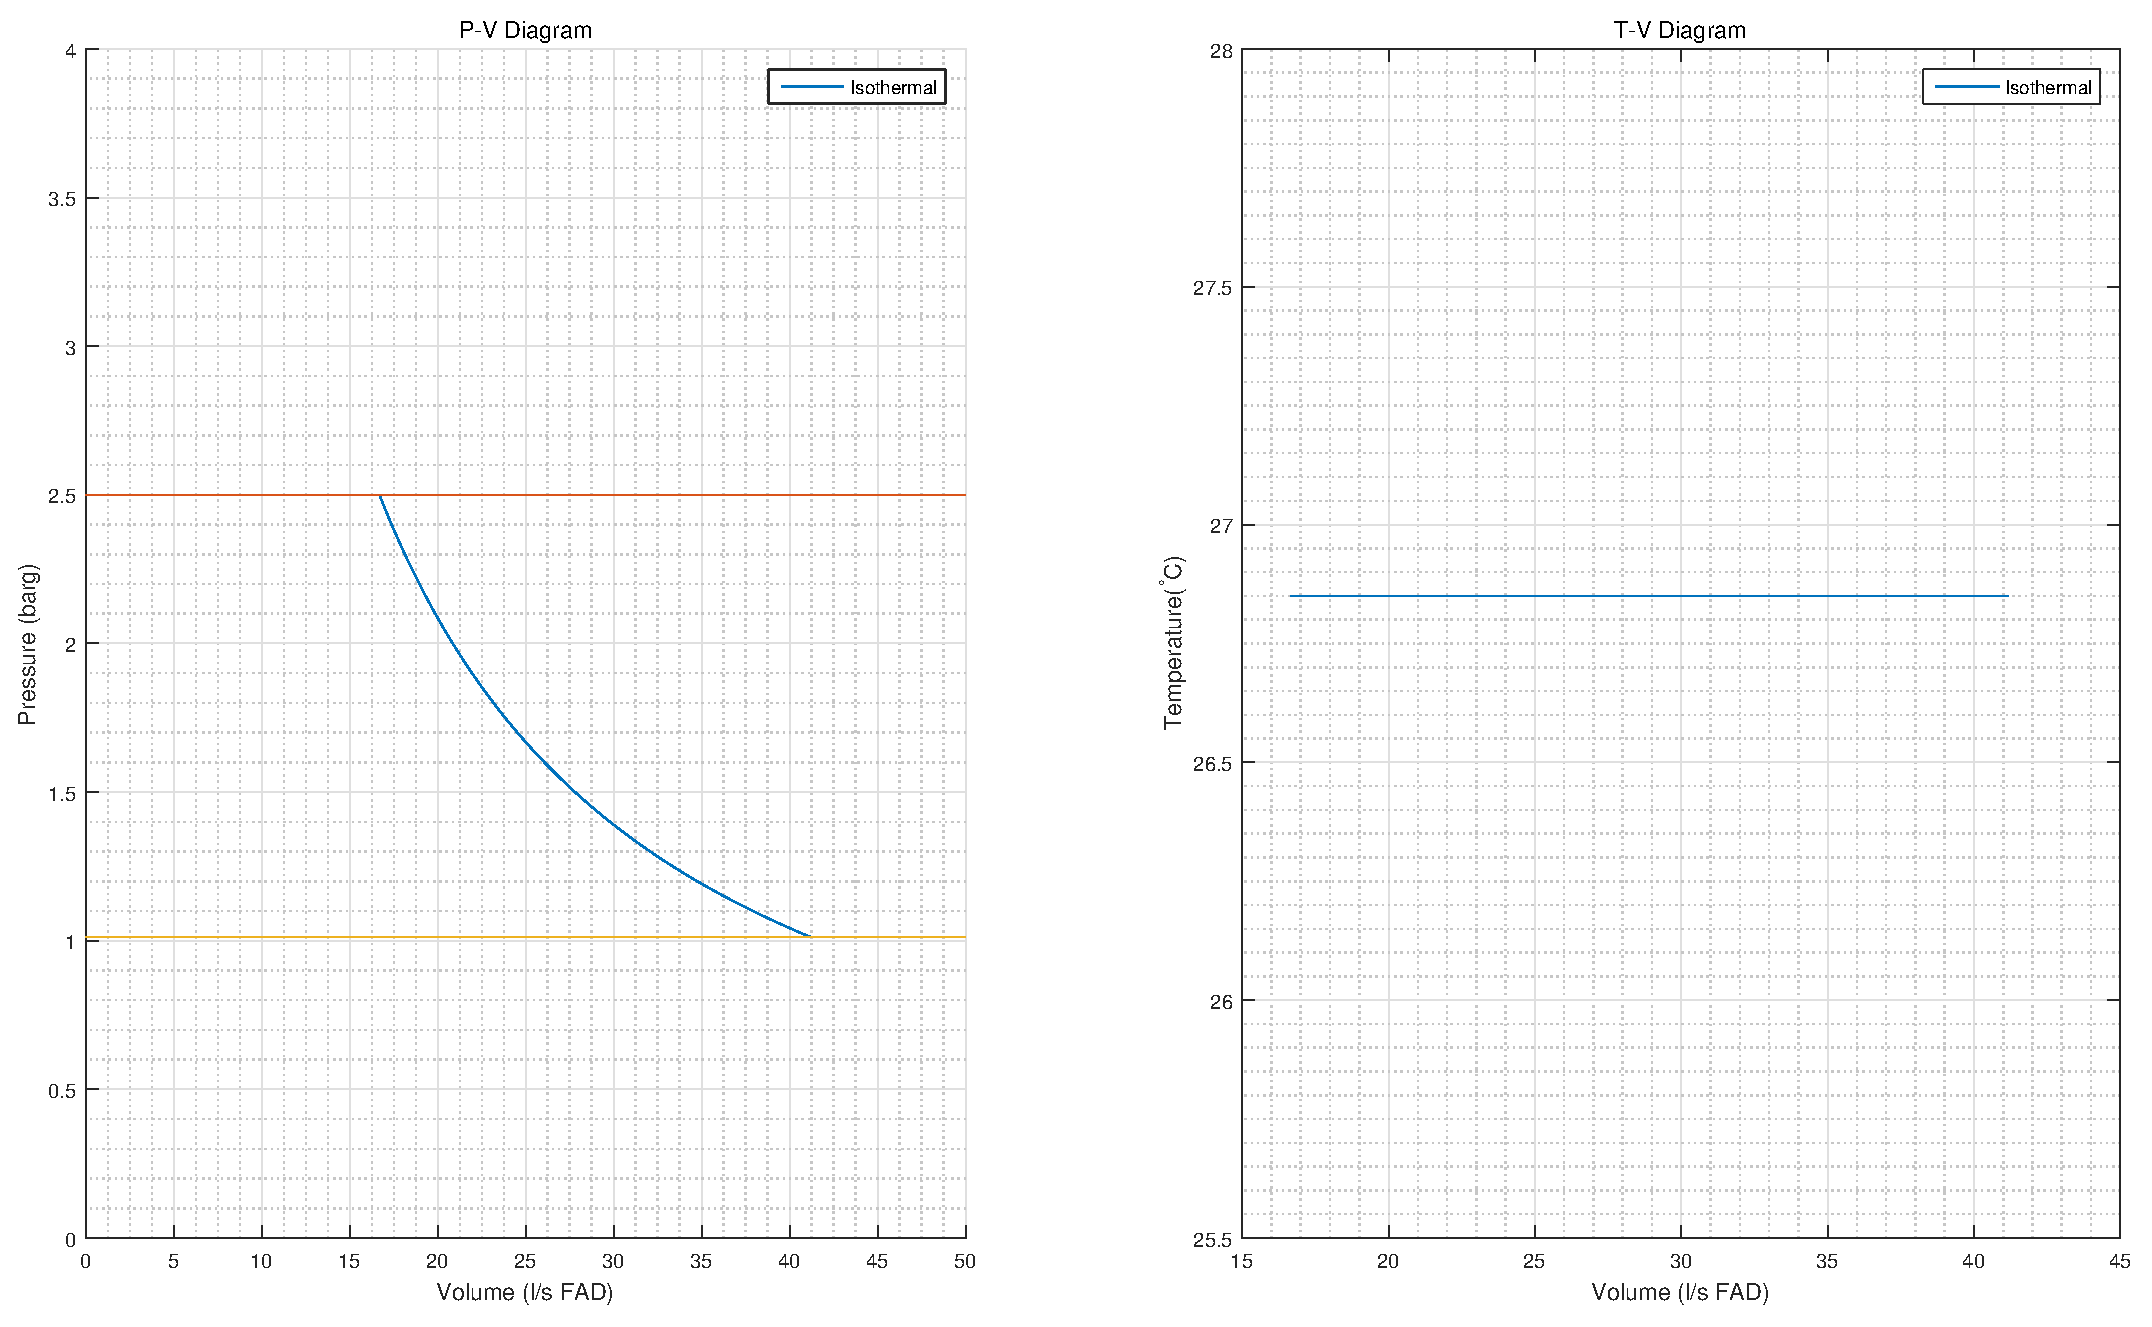
\includegraphics[width = \textwidth]{IsothermalCompressionOneStage.eps}
\caption{Isothermal Compression}
\label{fig:isothermalcompression}
\end{figure}

\section{Adiabatic Compression}
For adiabatic compression, no heat is transferred between the system and its surroundings. Furthermore if the process is idealised to be reversible (i.e. frictionless) the process is said to be adiabatic.

For this type of compression the following relationship holds true:

\begin{equation}
PV^{\gamma} = Constant
\end{equation}
In this equation. $\gamma$ refers to the specific heat ration $\left[ \frac{C_{p}}{C_{v}} \right] $ of air. This value is dimensionless and is 1.4 for air.

Therefore for the initial conditions above we can calculate:

\begin{equation}
101,325 * 0.0412^{1.4} = Constant (C) = 1,165.66
\end{equation}

We can therefore calculate the volume of the gas as it is compressed to 2.5 barg using:
\begin{equation}
V = \left( \frac{C}{P} \right) ^{\frac{1}{\gamma}}
\end{equation}

Using \autoref{eq:combinedgaslaw} we can calculate the temperature as the pressure increases and the volume decreases.

\end{document}